This chapter lays the foundational knowledge required for the reader to comprehend the subsequent chapters of this thesis. First, it will be presented the general scenario of cloud computing in Section~\ref{sec:cloud}. Then, an introduction to scheduling in the scenario of clouds will be shown in Section~\ref{sec:scheduling_cloud}. Finally, the question of the environmental impact and exisitng approaches will be discussed in Section~\ref{sec:carbon_responsive}, as well as state-of-the arts studies that were used in this thesis as inspiration and baselines.

\section{Cloud computing}

\label{sec:cloud}

Cloud computing was introduced by the industry to address the most significant problems of e-commerce found at the time. Before the on-demand access to computational resources provided by cloud computing, when a user or company wanted to deploy their service or application it would be necessary to buy his own computational infrastructure, and in the situation of a sudden peak of requests, it might not be possible to not scale at time to handle the computational load demand. Despite its revolutionary aspects of information technology, cloud computing is not classified as a new paradigm in computer science research. As a matter of fact, it is the evolution of research into different fields of computer science, such as clusters, grids, autonomous computing, ubiquitous computing. 

One of the critical elements that enables cloud computing is the virtualization technology: the computational resources of a physical machine are converted to virtual resources that can be shared among many users and applications --- also know as multitenancy.  The main ideas from virtualization originates from the late 1950's and beginning of 1960's with the multiprogramming paradigm, and today the reserach on virtual machines (VMs) and containers continue to investigate the compromises outlined in the literature of multiprogramming in terms of portability --- allowing the virutal resource to execute in any hardware,  performance --- the impact of additional virtual layer in the application execution in comparison to the gains regarding the multitenancy, and security --- how to isolate the interaction between different applications and the applications and the computational resources \cite{randall2020_virtualization}.

Cloud computing platforms generally support services in three distinct levels: IaaS (Infrastructure as a Service), PaaS (Platform as a Service) and SaaS (Software as a Service) \citep{fos08}. In the first level, Infrastructure as a Service (IaaS), the platforms grants the user access to hardware resources (such as processing and storage) and charge them for their usage. Services as Amazon EC2 (Elastic Cloud Computing) Service and Amazon S3 (Simple Storage Service) are examples of IaaS clouds.   At the second level, Platform as a Service (PaaS), the provider supports complete development, testing, and deployment environment for the application developer, which usually means that the developer will have to follow a specific fixed development model and accept restrictions on how to model the software in exchange for the scalability provided. An example is the Google App Engine.  Finally, at the third level, Software as a Service (SaaS), specific applications are offered to users via the Internet and the rate is proportional to the use of the application. We can cite as examples as Google Docs office applications.

Modern cloud computing platforms are composed by multiple data centers geographically distributed over the world --- also denominated cloud federations or multi-clouds. Figures illustrates the locations of the cloud data centers from Microsoft's Azure that in total consists of hundred of physical servers. The need for such geographically distributed infrastructre comes from meeting the demand of the huge number of users and reducing the response time for their aplications, as well for security and redundancy reasons, for example, if a data center on a region goes down by a power problem or hacking attack, other region could temporarily receive the computational load. Finally, this distributed infrastructre enables exploring differents approaches to reduce the environmental impact of operating the data centers, and more deatils of these strategies will be given in Section~\ref{sec:carbon_responsive}.


\begin{figure}[h]
\centering
  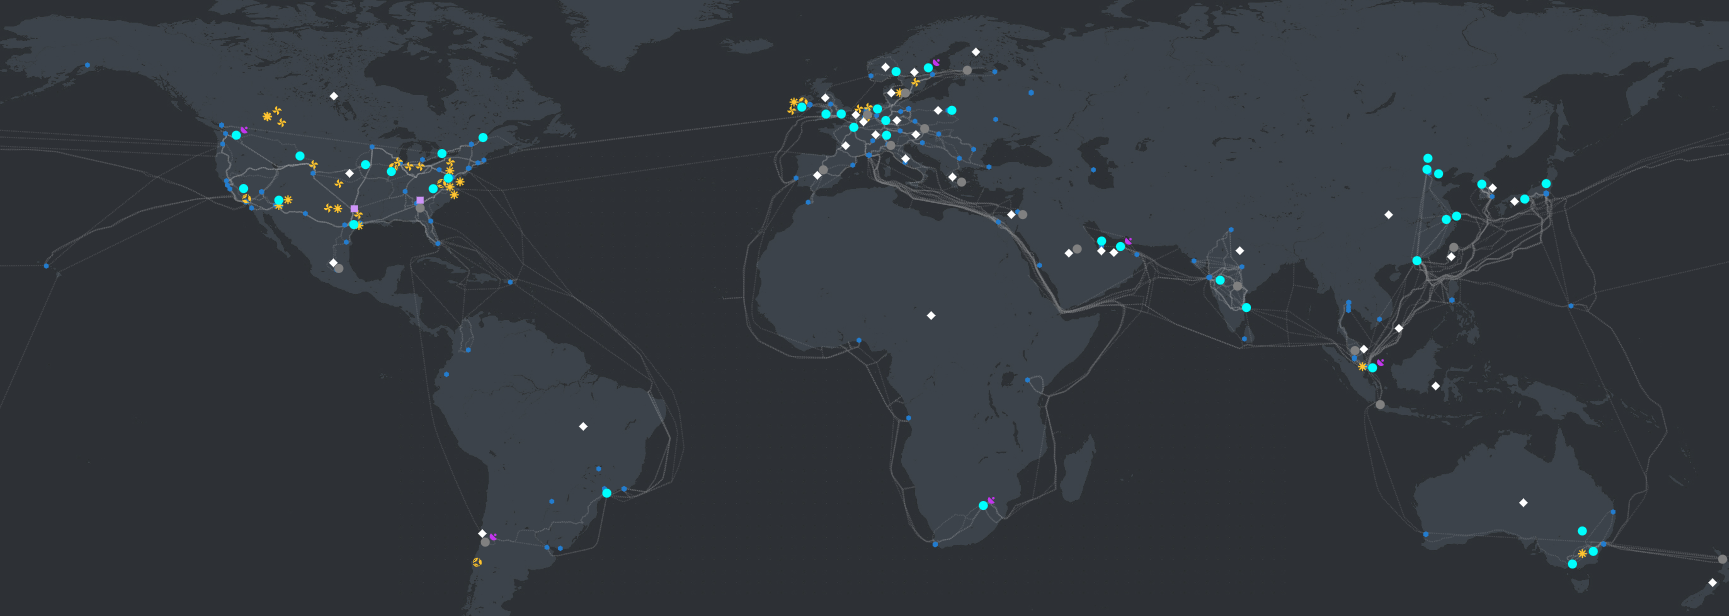
\includegraphics[width=\linewidth]{images/azure_cloud_infra.png}
  \caption{Locations of Microsoft's Azure Data centers.}
  \label{fig:dc_locations}
\end{figure}


\section{Measuring the environmental impact of cloud computing platforms}

- metrics

- falar dos 3 escopos la 


\section{Scheduling for cloud computing platforms}
\label{sec:scheduling_cloud}

Scheduling problems are combinatorial optimization problems where, given the description of the characteristics of a computational resource set ($\alpha$) and a task set ($\beta$), the objective is to find an allocation (in time) of resources to tasks that minimize some optimization criteria ($\gamma$). These problems are denoted, generally, using the $\alpha$ $\vert$ $\beta$ $\vert$ $\gamma$ notation, introduced by Graham \citep{graham}. 

The most common criterion studied in problems of high-performance computing is called makespan (also denoted by $C_{\max}$), which indicates the time when the last task that makes up an application finishes its execution. When the available computational resources are identical and known previously, and we are interested in minimizing makespan---typically the case in scheduling problems in cluster clusters and computational grids---the problem is strongly NP-complete \citep{Garey}. This problem is denoted by $P\,\vert\,\vert\,C_{\max}$ in Graham's notation.

For the research problem explored in this thesis, $\alpha$ represents the computational resources (memory and CPU) from the servers of the data centers as well as their information about availability of low-carbon intensive power sources, $\beta$ represents the VM requirements in terms of execution time,  deadline, memory and CPU, and $\gamma$ represents the reduction of carbon-intensive energy consumption.

It is known---from the work of \citet {graham} and \citet {Garey}---that the class of greedy algorithms known as list algorithms provides fast and efficient heuristics for scheduling tasks on parallel computers. These algorithms have a $2 -1 /m$ approximation guarantee for the worst case, but are remarkably effective in practice, especially when the ratio of the number of tasks to the number of available computational resources is large. Among the most commonly used list algorithms are the Longest Processing Time first (LPT) and Shortest Processing Time first (SPT),  for homogeneous platforms, and the Heterogeneous Earliest Finish Time (HEFT) algorithm, for heterogeneous platforms.


% TODO exemplos de coisas com scheduling, falar da consolidacao, migrar as vms sem preemption live migration ...


In particular, DCs can apply VM consolidation techniques in order to relocate the VMs into the smallest number of physical machines and turn off the idle
machines. \cite{10.1145/3470972} present a systematic literature review on such techniques.


The greedy algorithms were adopted in the solutions proposed in this thesis as well as most of the related works used as baseline and inspiration. The justification for such decision is that despite not providing the optimal solution, they can provided an acceptable solution in a reasonable amount of time, which is important considering the size of the workload with millions of tasks and restrictions as deadline, response time, and others. In the next section the reader will be presented to these strategies.


\section{Carbon-Responsible Computing}

\label{sec:carbon_responsive}

Many efforts from both academia and industry are being made to reduce the environmental impact of information technology. The term Carbon-Responsive Computing was created to describe the strategies that explores moving the computational workload both in the time and spation dimensions aiming to reduce the carbon footprint of the operation~\cite{schooler2021carbonaware}.

There are three levels for Carbon-Responsive computing. In the first, Carbon-aware computing, the system knows the carbon intensity of the electricity used by its workloads or IT equipments. On the second, Carbon-responsive computing, the information about the carbon intensity is taken into account to make decisons. On the final stage, Carbon-resilient computing, it is studied how to manage and integrate carbon-responsive elements and what modifications are needed in the infrastructure for both IT and power supply.

In this thesis, it is presented a study of the Carbon-Aware strategy follow-the-renewables --- presented in Section~\ref{sec:followtherenewables}, and the Carbon-Reslient computing strategy of sizing the renewable infrastructure --- discussed at Section~\ref{sec:sizing}.

\subsection{Follow-the-renewables}

\label{sec:followtherenewables}

What is follow the renewables ???


Large hosting and Cloud Computing providers have DCs distributed on
different geographic locations---some of them on different time
zones---in order to provide services with low latency and high
availability. Scheduling algorithms can take advantage of this to
mitigate the intermittent availability of renewable energy by
redistributing the workload based on renewable energy
availability. This idea is known in the literature as the
``follow-the-renewables'' \cite{shuja2016sustainable}. 



\cite{XU2020191} present a comprehensive overview of the classical
techniques used for reducing the energy consumption on DCs. They also
introduce a workflow shifting algorithm that redistributes the
workload among different DCs located in different time zones. The
objective of their algorithm is to minimize the total carbon emission
while ensuring the average response time of the requests. In their
work, jobs are initiated in the selected DCs instead of migrated after
starting its execution, and there is no server consolidation.


Minimization of energy consumption, costs, and environmental impact
while ensuring the workload performance were studied
by~\cite{ALI2021110907}. They proposed a solution that manages
geographic distributed DCs with heterogeneous servers in a distributed
fashion. The solution has two main algorithms that use greedy
heuristics: the first performs the allocation of the incoming workload
to the servers of the DCs according to a defined policy (lower energy
prices or more available green power); and the second either migrate
the workload only among the servers inside a DC (intra-DC migration)
to reduce the number of utilized servers, or migrate the workload
among different DCs (inter-DC migration) according to an arbitrary
policy (use the DCs with lower electricity price, or more green power
available). The migrations in the second algorithm can result in a
decrease in performance, given that a task could be migrated to a
server that is not as powerful as the one where it was running before
being migrated, and the proposed solution considers this metric.



- falar do nemesis e scorpius


``Follow-the-renewables'' is an interesting solution for mitigating
the intermittency of renewable energy availability, but it also has
limitations. First, the process of migrating a VM between different
DCs consumes energy itself. The scheduling algorithm must consider
this energy consumption before deciding if the migration is
advantageous. Second, the network communications links between the DCs
can suffer from contention, which may increase the execution time of
the jobs, migration duration, and costs. An efficient scheduling
algorithm must consider those factors to decrease the carbon footprint
of the DCs operations.


\subsection{Sizing the renewables infrastructure}

\label{sec:sizing}


Most sizing research focuses on a single DC. There are two approaches, either to consider that the DC can use the electrical grid as a fallback or to consider how to size a DC only with on-site renewable sources.

Most sizing approaches consider the capability to use the electrical grid. %sizing with grid
\cite{padma2021_fogdcs_rural} use a Particle Swarm Optimization approach for sizing a smart microgrid to supply fog DCs located in a rural area in India. The objective of the optimization is to reduce the capital cost of buying solar panels, wind turbines, diesel generators, and batteries. Power from the regular electrical grid can be used when there is no green power production. The authors also propose a scheduling algorithm to maximize green energy usage.
% https://doi.org/10.1007/s11276-019-02207-z
%
\citet{Niaz2022_curtailment} evaluates using curtailed renewable energy to power DCs and provide hydrogen to hydrogen refueling stations. The authors model their problem as a MILP (Mixed Integer Linear Programming) with the objective of minimizing the costs. System components included natural-gas–powered combined cooling, heating, and power systems, electrolyzers, hydrogen fuel cells, heat pumps, hydrogen tanks, and battery energy storage systems. The results were that using only power from the electrical grid was the worse in both economic and environmental terms. Using a mix of curtailed renewable energy and electricity from the grid was the most economical. Using only renewable energy was the best for the environment; however, it had the highest costs.
% https://doi.org/10.1016/j.jpowsour.2022.231558

%sizing without grid
In some cases, the approach considers how also to size on-site energy production, removing the need to access the electrical grid.
\citet{Richter2021_netzero_dcs} proposes a planning methodology for net-zero energy systems, and performed a qualitative study to evaluate a net-zero energy DC located in Germany. The conclusion is that by selecting appropriate technologies for energy generation, increasing energy efficiency, and optimal sizing Energy Storage Systems, the DC showed large potential to operate as a net-zero energy system. A DC as a net-zero energy system can increase the marketing image and add economic value to the related company.
% https://doi.org/10.3390/en14175577
%
\citet{HADDAD2021100505} proposes to size a DC using only on-site renewable energy and energy storage systems (batteries and hydrogen). This work focuses on a single DC and discusses the impact of its location, its workload, and its context on the resulting sizing (number of servers, renewable sources, and storage).
% https://doi.org/10.1016/j.suscom.2020.100505
%
\citet{manal2022} proposes to reduce the usual oversizing of renewable-powered DCs. Classical sizing approaches based on traces are defined by a few days with unusually high workloads and/or low renewable availability. In this work, the authors propose to reduce such sizing and evaluate the impact on the Quality of Service and on the sizing itself. Contrary to the previous studies, they use a binary search approach to find the best relevant sizing instead of MILP formulation.

%elec sizing
Some research focuses on the sizing of particular elements, such as the electrical infrastructure.
% \citet{Kazhamiaka22_comparison_pv_bat_sizing} evaluates the state-of-the-art in sizing both PVs and batteries simultaneously with the minimum cost. They consider optimization methods, simulations, and stochastic network calculus. The conclusion is that simulation appears to be the best too for sizing, due to both qualitative and quantitative reasons.
% https://doi.org/10.1109/TSUSC.2019.2946246
% not related to DC sizing, we can use the space to talk about the carbon explorer work
%
\citet{sheme2018_batsize} studies the impact of the battery size to reach a specific green coverage of 50\% (half of the energy consumption of the DC needs to be green). They develop a simulation tool that uses as input the area of PVs and capacity of the batteries. Experiments comparing countries (Finland, Crete, and Nigeria) show that the number of solar panels needed in Crete and Finland is slightly higher than in Nigeria, 17\% and 45\%, respectively. However, although Finland provides only 15\% less annual solar energy than Nigeria, it requires a battery size of 39 times bigger to achieve wasted energy at level 0. While in Crete, a battery capacity of only 27\% greater than in Nigeria is needed. %for this goal.}
% https://doi.org/10.1007/978-3-319-75928-9_49


Overall, most studies focus on sizing individual DCs. This is similar in the context of scheduling renewable-powered DCs: \citet{SONG2022326} reviews recent publications on the field of DCs powered by Renewable Energy mix. It shows that among more than 100 publications, only a quarter focuses on geographically distributed data centers partially powered by renewable energy mix. It also shows that most research in this field focuses on workload scheduling, while few articles focus on the adaptation or sizing of the infrastructure.

% The Carbon Explorer work from Facebook is similar and very related to this paper. It should be discussed in the related work at least.

The Carbon Explorer framework is an example of a study that explores sizing multiple DCs \cite{acun2022holistic}. The framework explores three solutions to achieve 100\% renewable operation of DCs distributed over the United States of America: i) only use renewable energy; ii) use renewable energy and energy storage; and iii) use renewable energy and schedule the workload. These DCs already have access to local solar power, wind power, or both. The carbon emissions from manufacturing PVs, wind turbines, batteries, and servers are considered. An exhaustive search is used to find the solutions. The work concludes that 100\% renewable operation may not be the optimal solution when considering the geographic location of the DC, and the carbon emissions from the manufacturing phase. Furthermore, the authors say that choosing the optimal solution is still an open research question for future work.


Our approach focuses on optimally sizing of geo-distributed DCs across the globe, which has not yet been studied to the best of our knowledge. Furthermore, in contrast to the Carbon Explorer framework, our solution allows using the regular electrical grid when opportune, given it may be supplied by a low-carbon intensive source. Finally, contrary to most studies using a MILP, our model uses a linear program formulation.



%% Add about chasing carbon  - https://doi.org/10.1109/MM.2022.3163226

%% Add about ACT: designing sustainable computer systems with an architectural carbon modeling tool -  https://doi.org/10.1145/3470496.3527408

% TODO:: add as reviews la de coisas verde q o daniel mandou

\section{Summary}


In this chapter we presented a brief overview of the scheduling theory in the context of High Performance Computing, with emphasis on parallel job scheduling problems, list scheduling and backfilling algorithms. We also made a short introduction to machine learning, with emphasis on regression problems. Finding optimal solutions for parallel job scheduling problems is notoriously hard and, although there are many approximation algorithms with proven performance guarantees, many practitioners end up adopting simple heuristics, such as EASY Backfilling, to schedule parallel jobs. The content present in this chapter must be sufficient for the reader to follow the remaining chapters of this thesis. In the remaining chapters we present the main contributions of the thesis, starting by presenting the ways we explored simulation and machine learning to learn simple parallel job scheduling heuristics. 